\documentclass[../../Thesis.tex]{subfiles}

% “  ”

\begin{document}
	
	\section{Simulation Tools}
			
		In this section, we will present the instruments, the techniques, and the robots' tasks that we have used to collect the simulation data for our tests.
		
		\subsection{Simulators}
		\label{sec:simulators}
			This project has been developed with data retrieved from two different simulators. The first simulator which has been used is ARGoS (Autonomous Robots Go Swarming), developed by Carlo Pinciroli \cite{Pinciroli:SI2012}, that is an open-source multi-robot simulator with the focus on real-time simulation of large heterogeneous swarm of robots. Thanks to its modular and open-source approach we have been able to easily modify the source code in order to implement the necessary simulations.  We can see a snapshot of the graphical user interface in Figure \ref{fig:ARGoS_gui_snapshot}.  In our simulations we used a software model of foot-bot agents which will be introduced in Section \ref{sec:Robot_description}.\\
			\begin{figure}
			    \centering
			    \includegraphics[width=0.8\textwidth]{../../Images/Data_collection/argos_gui_snapshot.png}
			    \caption{Snapshot of ARGoS graphical user interface.}
			    \label{fig:ARGoS_gui_snapshot}
			\end{figure}
			The second simulator which has been used is RAWSim-O (Robotic Automatic Warehouse Simulator (for) Optimization), developed by Marius Merschformann \cite{Merschformann2018}, that has been created to simulate a Robotic Mobile Fulfillment System (RMFS) and to study the impact on the performance of different decision strategies. We can see a snapshot of the graphical user interface in Figure \ref{fig:RAWSim-O_gui_snapshot}. The author does not specify a unique physical robotic agent for its environment but uses a conceptual implementation of the Kiva systems shown in Figure \ref{fig:RAWSim-O_bots}. The robots used in the RAWSim-O simulation are a software implementation of agents that are able to perform every action of a physical Kiva robot.
			\begin{figure}
			    \centering
			    \includegraphics[width=0.8\textwidth]{../../Images/Data_collection/rawsim-o-3d.png}
			    \caption{Snapshot of RAWSim-O graphical user interface.}
			    \label{fig:RAWSim-O_gui_snapshot}
			\end{figure}

		\subsection{Robot Description}
		\label{sec:Robot_description}%
			The foot-bot is shown in Figure \ref{fig:Footbot_photo}, and it can be referred to also as MarxBot \cite{Bonani2010}. They were developed within the EU-funded project Swarmanoid \cite{Swarmanoid2006}. The foot-bot is a miniature mobile robot that addresses the needs of having a large battery life, being able to perceive its peers, and being able to interact with them.  The robot measures 17 cm in diameter and 29 cm in height with a weight of 1.8 kg. The base module provides rough-terrain mobility thanks to a combination of tracks and wheels. The base module contains also proximity sensors, a 3-axis gyroscope, and a 3D accelerometer. A range and bearing module allows the robot to compute a rough estimate of the direction and the distance of the neighboring robots. A distance scanner allows the robot to build a 2D map of its environment. The on-board computer drives two cameras, one looking front and one oriented towards an omnidirectional hyperbolic mirror.\\
			\begin{figure}
			    \centering
			    \includegraphics[width=0.3\textwidth]{../../Images/Data_collection/footbot-final.jpeg}
			    \caption{Photo of Foot-bot.}
			    \label{fig:Footbot_photo}
			\end{figure}
			The RAWSim-O simulator requires a robot that is able to carry heavy inventory pods and the Foot-bot would not be adequate for this task. The RMFS simulated by RAWSim-O is similar to the management system of the Kiva systems \cite{Enright2011}, known also as Amazon Robotics.  An early version of Kiva's robots (Figure \ref{fig:Kiva_bot}) is composed of 5 main parts: navigation system, lifting mechanism, power system, collision detection system, and driving system \cite{Guizzo2008}. The navigation system is composed of a camera facing upwards, in charge of reading bar codes under inventory racks for identification, and of a camera facing down that reads barcodes on the floor for navigation. The lifting mechanism consists of a large screw that lifts inventory racks 5 centimeters from the ground. The power system is composed of four batteries that are charged at the charging station. The collision detection system is composed of infrared sensors and touch-sensitive bumpers. The driving system is made of two brushless dc motors that control independent neoprene rubber wheels making the robots move at 1.3 $\frac{m}{s}$. Physical experimental simulations of small warehouse environments have been deployed using a vacuuming robot \cite{IRobot}.  The robots are equipped with ASUS Eee PCs, webcams for line-following, a blinking light for visual feedback, and RFID tag readers for waypoint recognition. The maximum velocity of the vacuuming robot is 0.21 $\frac{m}{s}$, while a complete turn takes 5.5 $s$. Maximum acceleration and deceleration are 0.5 $\frac{m}{s^2}$ and -0.5 $\frac{m}{s^2}$. A photo of the Kiva can be seen in Figure \ref{fig:Kiva_bot}. A photo of the demonstrator setup can be seen in Figure \ref{fig:RAWSim-O_demonstrator}.
			
			\begin{figure}
			    	\centering
			    	\subfloat[RAWSim-O demonstrator bot.
			    		\label{fig:RAWSim-O_demonstrator}]{
			    		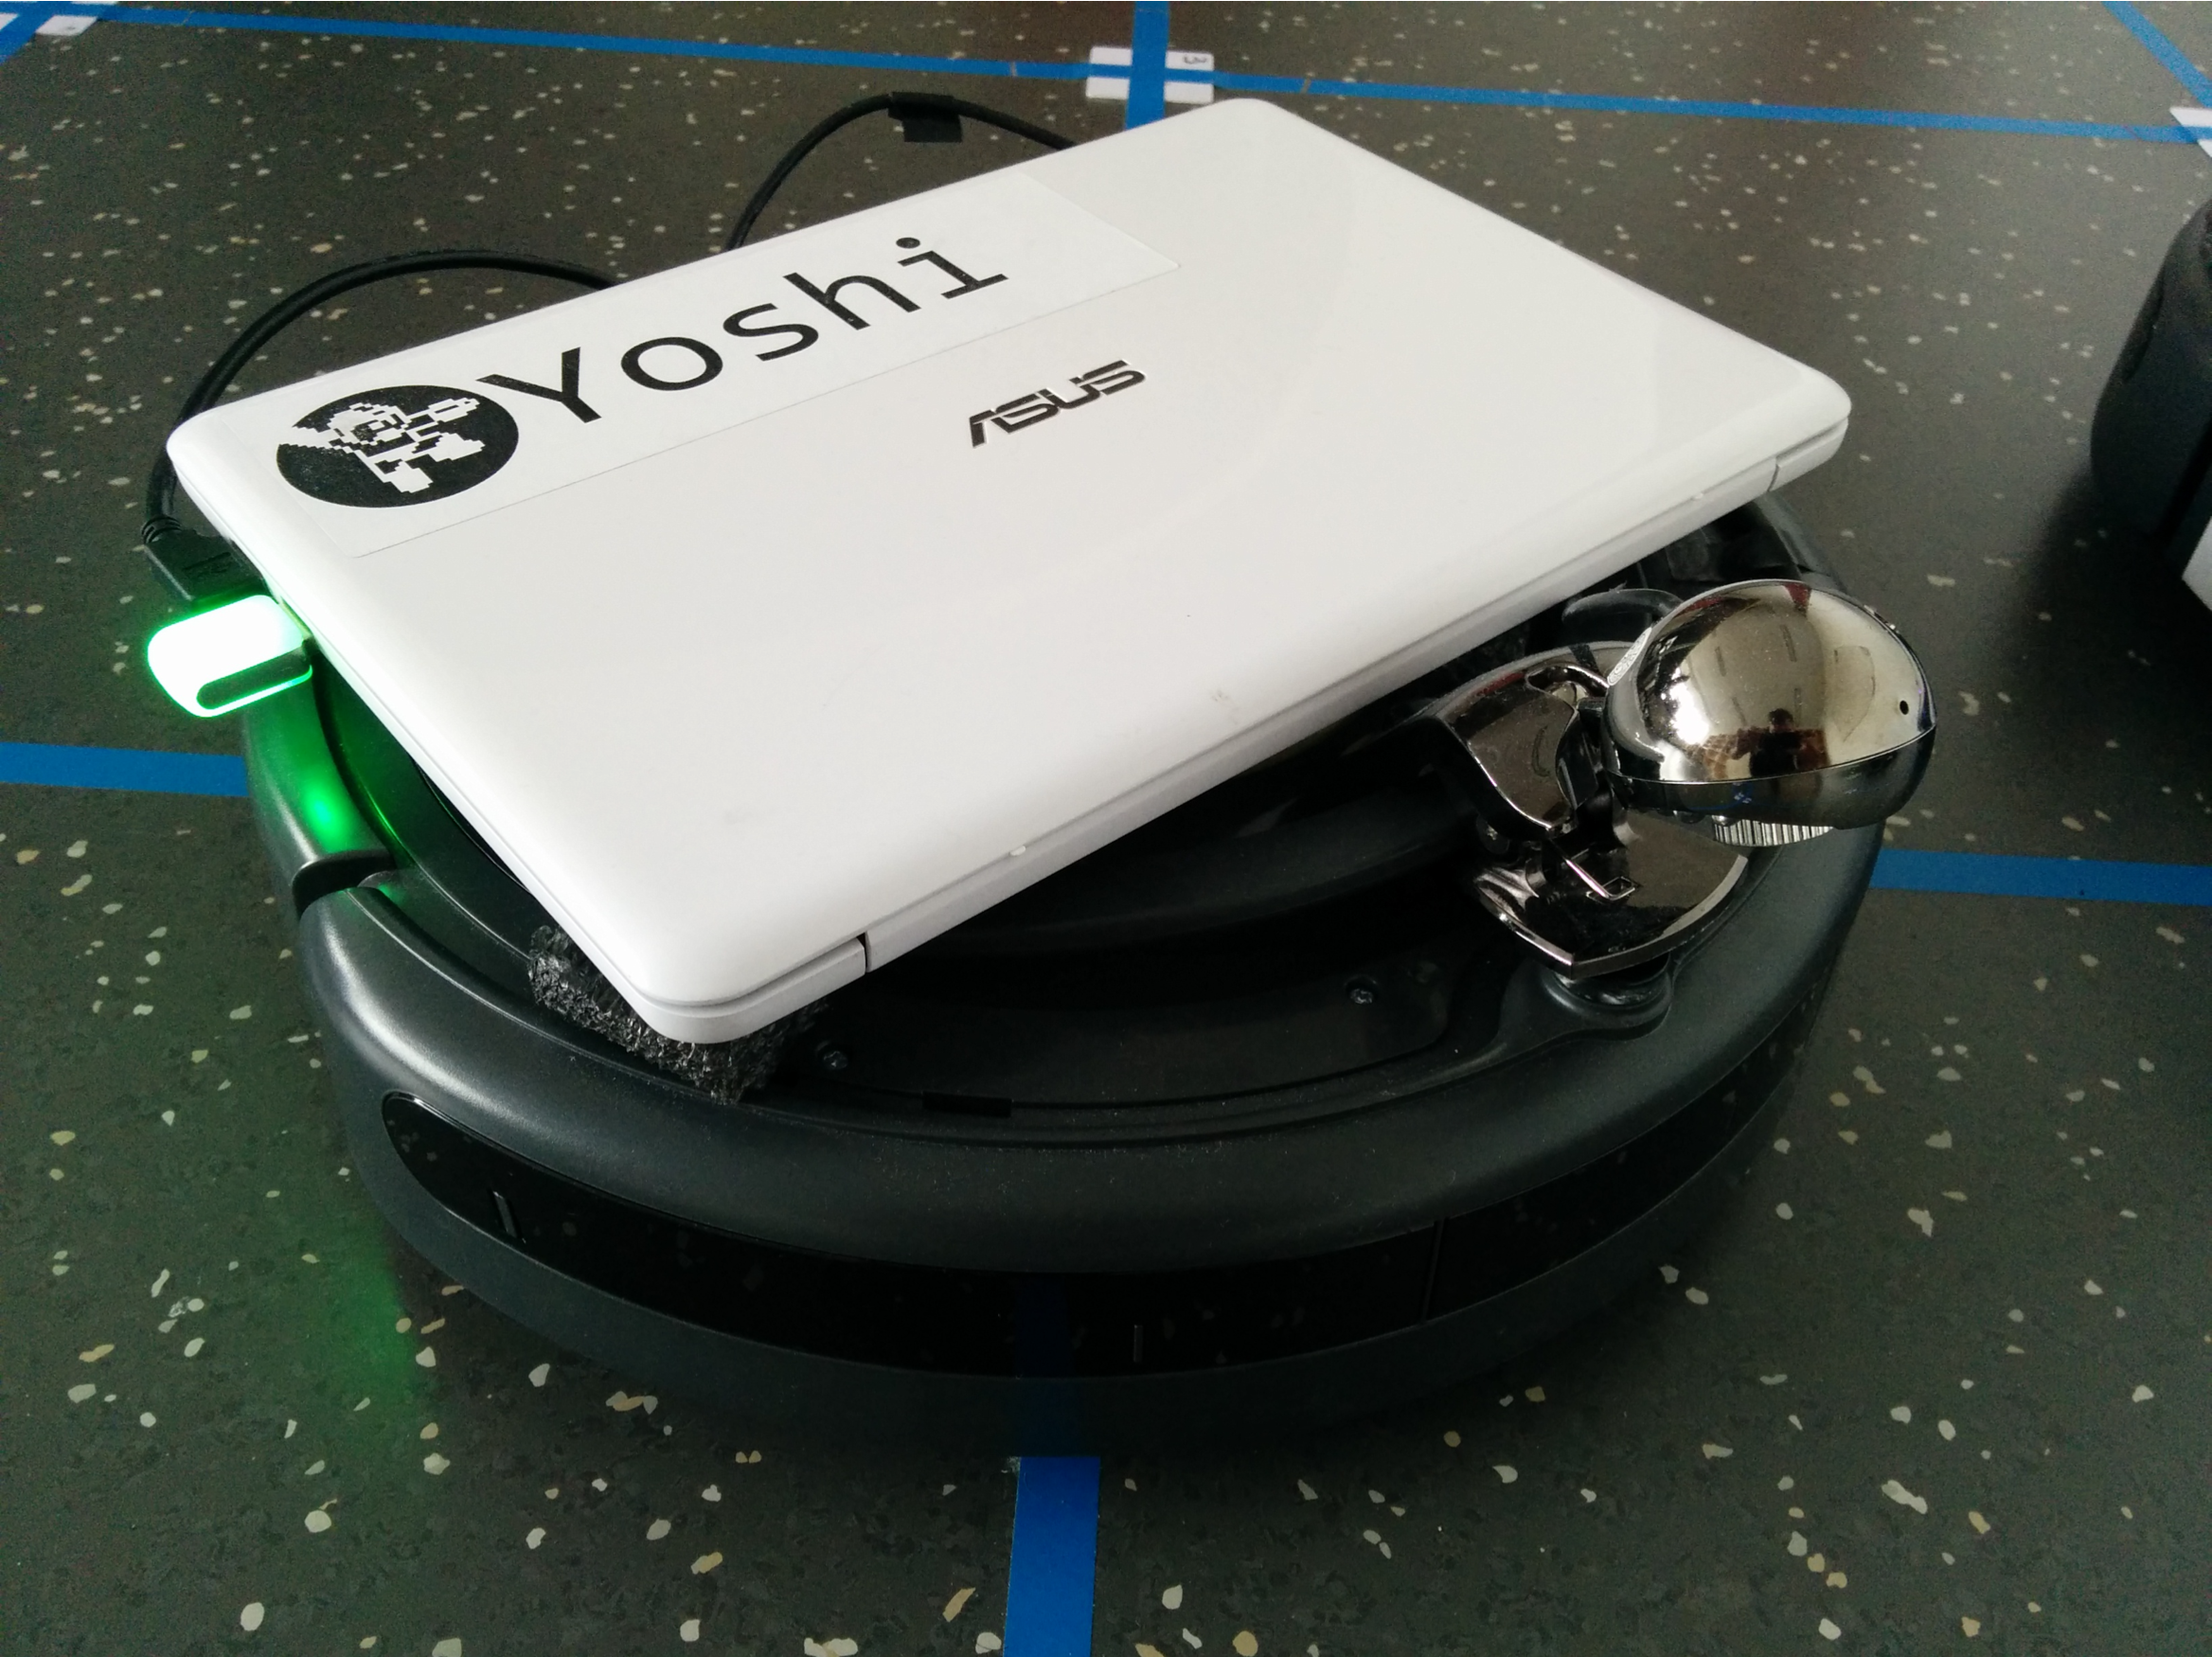
\includegraphics[scale=0.2]{../../Images/Data_collection/RAWSim-O_demonstrator_robot.png}
			    }
			    \quad
			    \subfloat[Kiva robot carrying inventory pod. \label{fig:Kiva_bot}]{
			        \includegraphics[scale=0.23]{../../Images/Data_collection/Kiva_robot_inventory_pod.png}
			    }
			    \caption{RAWSim-O bots.}
			    \label{fig:RAWSim-O_bots}
			\end{figure}
			
			In the following sections, we will explain the mechanism behind each task behavior and show the principal characteristics of the task.
		\subsection{Flocking}
		\label{sec:Flocking}%
			The flocking task we refer to is the one introduced by Ferrante et al. in \cite{Ferrante2012}. By its definition, flocking is the “cohesive and ordered motion of a group of individuals in a common direction”. Ferrante et al. proposes a magnitude dependent motion control (MDMC) to “achieve flocking with minimal components”. A snapshot of flocking execution can be seen in Figure \ref{fig:ARGoS_flocking}.\\
			\begin{figure}
			    \centering
			    \includegraphics[width=0.5\textwidth]{../../Images/Data_collection/ARGoS_flocking_snapshot.png}
			    \caption{Snapshot of flocking task execution.}
			    \label{fig:ARGoS_flocking}
			\end{figure}
			The method used to achieve flocking is composed of different components: proximal control, alignment control and motion control. The main concept behind this method is that each robot computes a flocking vector
			\[\mathbf{f} = \mathbf{p} + \mathbf{a} + \mathbf{g}\]
			where:
			\begin{itemize}
				\item $\mathbf{p}$ is the proximal control vector in charge of the attraction and repulsion forces.
				\item $\mathbf{a}$ is the alignment control vector in charge of the alignment rule.
				\item $\mathbf{g}$ is the goal direction vector in in charge of the goal following behavior.
			\end{itemize}
			\subsubsection{Proximal Control}
				Proximal control computes all the forces needed to keep each robot at a certain distance from its neighbors. The proximal control rule encodes the attraction rules, to shorten the distance between neighbors, and the repulsion rules, to move further away robot that are too close. Proximal vector is computed as:
				\[\mathbf{p} = \sum\limits_{i = 1}^{m_p} p_i(d_i) e^{j \phi_i},\]
				where:
				\begin{itemize}
					\item $p_i(d_i) e^{j \phi_j}$ is a vector in the complex plane, its formula is defined in \citep{Ferrante2012}.
					\item $m_p$ is the number of neighboring robots perceived in the range $D_p$.
					\item $d_i$ is the relative range computed from the body-fixed reference frame.
					\item $\phi_i$ is the bearing of the $i$-th neighboring robot.
				\end{itemize}
			\subsubsection{Alignment Control}
				Alignement control computes the average orientation of the robot's neighbors and adjusts the robot's orientation accordingly. The alignment control method uses the following formula:
				\[\mathbf{a} = \frac{\sum\limits_{i=0}^{m_a} e^{j\theta_i}}{\left| \left| \sum\limits_{i=0}^{m_a} e^{j \theta_i}\right|\right|},\]
				where:
				\begin{itemize}
					\item $\theta_0$ is the orientation of the focal robot, namely the current robot.
					\item $m_a$ is the number of neighbors within a range $D_a$ of the focal robot.
					\item $\theta_i : i \in \lbrace 1, \dots, m_a \rbrace$ are the orientations of the neighbors.
					\item The operator $|| \cdot ||$ denotes the length of a vector.
				\end{itemize}
			
			\subsubsection{Motion Control}
				Motion control has to convert the flocking vector into forwarding speed $u$ and angular speed $\omega$. The model proposed by Ferrante et al. identifies as $\mathbf{f}_x$ and $\mathbf{f}_y$ the projections of the vector $\mathbf{f}$ on the $x$-axis and the $y$-axis respectively. $\mathbf{f}_x$ determines the forward speed $u$, while $\mathbf{f}_y$ determines the angular speed $\omega$. The model equations are:
				\begin{align*}
					u & = K_1 \mathbf{f}_x + U \\
					\omega & = K_2 \mathbf{f}_y,
				\end{align*}
				where:
				\begin{itemize}
					\item $U$ is a forward biasing speed.
					\item $K_1$ and $K_2$ are linear and angular gains respectively.
				\end{itemize}
		
		\subsection{Foraging}
		\label{sec:Foraging}%
			To describe the foraging we refer to \cite{Winfield2009} and the code used in the ARGoS simulator. The foraging task is broadly defined as searching for, collecting, and returning resource items to a point of delivery or nest area. This behavior can be seen as a heterogeneous task composed of several actions such as exploration, harvesting, resource transportation, and homing. Foraging robots are mobile robots capable of searching and transporting objects to a collection point. This task can be executed by single robots or multiple robots operating collectively. A snapshot of the foraging task can be seen in Figure \ref{fig:ARGoS_gui_snapshot}.\\
			The finite state machine represented in Figure \ref{fig:fore_FSM} summarizes the control algorithm used in \cite{PinciroliCode}. The robot is always in one of four states: resting (Rest), exploring (Expl), homing (Home), searching for space in nest (Nest). In our experiments, there are multiple target objects, namely resources to collect, which continuously regenerate, and a unique nest area where collected objects are deposited. Each robot has two internal variables: \verb|RestToExploreProb| defines the probability of transitioning from resting state to exploring state; \verb|ExploreToRestProb| defines the probability of transitioning from exploring state to resting state.
			\subsubsection{Resting}
				This is the initial state where all the robots start from the nest area. It is a state where the robots are in a sleepy state, they can only perceive the communications received from their neighbors and update the internal variables. After a robot has spent an amount of time greater than \verb|MinimumRestingTime|, if the random extraction from a uniform probability function is greater than \verb|RestToExploreProb|, then the robot changes state to exploring, otherwise it stays in resting state.
			\subsubsection{Exploring}
				In this state, the robot is performing a random walk while performing obstacle avoidance. During this behavior the robots can not use its sensors (front facing camera, omndirectional camera, range and bearing module) to look for the resources sparse in the arena, they can not communicate with their neighbors where other resources are, and it has not any specific place to reach. The random walk behavior is self-explanatory, the robot does not follow a predefined direction but randomly changes where it is headed. A robot detects a resource when at least two of the robot's floor sensors detect the color black. Once a robot has located a resource, it proceeds on grabbing it and it transitions to homing state. After a robot has spent an amount of time greater than \verb|MinimumUnsuccessfulExploreTime|, if the random extraction from a uniform probability function is greater than \verb|ExploreToRestProb|, then the robot changes state to homing, otherwise, it stays in exploring state.
			\subsubsection{Homing}
				In this state, the robot follows the signal emitted by the beacon that indicates the position of the nest area. The nest area is reached whenever the two ground sensor on the back perceives the nest area color on the floor. Whenever the robot reaches the nest area it drops the collected resource and transitions to searching for place in nest state.
			\subsubsection{Searching for Place in Nest}
				To avoid the positioning of all the robots on the border between the nest area and the area where resources are scattered, the algorithm forces the robots to spend some time searching for place in the nest.  When a robot has spent \verb|MinimumSearchForPlaceInNestTime| searching for a place in the nest, it communicates the result of its last exploration attempt to its neighbors and it changes its state to resting. 
			\begin{figure}
			    \centering % centers the figure
			    \begin{tikzpicture}
		        % tikz code goes here
			    	\tikzset{
			        ->,  % makes the edges directed
			        >=stealth', % makes the arrow heads bold
			        node distance=3cm, % specifies the minimum distance between two nodes. Change if n
			        every state/.style={thick, fill=gray!10}, % sets the properties for each ’state’ n
			        initial text=$ $, % sets the text that appears on the start arrow
			        };
			        \node [state, initial, accepting] (Rest) {Rest};
			        \node [state, accepting, right of=Rest] (Expl) {Expl};
			        \node [state, accepting, below of=Expl] (Home) {Home};
			        \node [state, accepting, left of=Home] (Sea) {Nest};
			        \draw (Rest) edge (Expl)
			        			 (Expl) edge (Home)
			        			 (Home) edge (Sea)
			        			 (Sea) edge (Rest)
			        			 (Expl) edge[loop above] (Expl)
			        			 (Rest) edge[loop above] (Rest);
			    \end{tikzpicture}
			    \caption{Foraging task finite state machine}
			    \label{fig:fore_FSM}
			\end{figure}
		
		\subsection{Robot Mobile Fulfillment System}
		\label{sec:Data_collection:Robot_Mobile_Fulfillment_System}
			The main innovation that RMFSs have brought to the field of warehouse management is to bring the shelves to the operators instead of the operators going to the shelves. RMFS can be summarized in a few simple components:
			\begin{itemize}
				\item Movable shelves, called \textit{pods}, where inventory is stored.
				\item Storage locations where it is possible to store pods.
				\item Workstations where the pick order items are retrieved from the pods (\textit{pick stations}) or replenishment order items are stored in the pods (\textit{replenishment stations}).
				\item Mobile \textit{robots} which can move underneath pods and carry them to workstations.
			\end{itemize}
			The storage and retrieval process can be seen in Figure \ref{fig:RMFS_central_process}.  When a robot gets a replenishment order, it carries a selected pod to a replenishment station to fill. When a robot gets a pick order, it carries a selected pod to a pick station to deliver the requested items. The administration of an RMFS requires the solution of a set of optimization and allocation problems.  In the approach proposed in \cite{Merschformann2018}, the solution of the decision problems is decomposed in a series of subproblems:
			\begin{itemize}
				\item \textbf{Order assignment:} divided into replenishment order assignment (ROA) and pick order assignment (POA).
				\item \textbf{Task creation:} divided into pod selection, which in turn is divided into replenishment pod selection (RPS) and pick pod selection (PPS), and pod storage assignment (PSA).
				\item \textbf{Task allocation:} assignment of tasks to robots.
				\item \textbf{Path Planning:} planning of the paths.
			\end{itemize}
			
			\begin{figure}
			    \centering
			    \includegraphics[width=0.6\textwidth]{../../Images/Data_collection/RMFS_storage_and_retrieval_process.png}
			    \caption{The central process of a RMFS.}
			    \label{fig:RMFS_central_process}
			\end{figure}
			For more detailed information about all the subproblems and their description, the reader can refer to \cite{Merschformann2018}.
			A graphical representation of the simulation process can be seen in Figure \ref{fig:RMFS_graphical_simulation_process}. The simulation has to manage the update of the agents, the outsourcing of decisions to controllers, and the delivery of information to a visualizer. The framework of the simulation is composed of three layers of configuration: layout specification, scenario specification, and controller configuration. The \textit{layout specification} specifies all the positions and individual characteristics of all stations, the waypoint system for robot direction, and the robot themselves. The \textit{scenario specification} specifies the information about the scenario to simulate, like the simulation duration and settings about the inventory and order emulation. The \textit{controller configuration} specifies which setting to use for each decision problem and their parameters.\\
			The robot movements are simulated with linear acceleration and deceleration for straight movements and they're constrained to predefined paths. They can not perform curved movements so each robot must rotate on itself in order to change direction. We can see a picture that depicts a RMFS simulation made with RAWSim-O in Figure \ref{fig:RAWSim-O_gui_snapshot}.
			
			\begin{figure}
			    \centering
			    \includegraphics[width=0.5\textwidth]{../../Images/Data_collection/RMFS_simulation_process_graphical.png}
			    \caption{Overview of the simulation process in a RMFS.}
			    \label{fig:RMFS_graphical_simulation_process}
			\end{figure}
			
		\section{Fault Implementation}
			Different faults have been implemented in the two simulators: in ARGoS we have implemented a rotating fault in which the bots rotate around a fixed point in the arena due to one wheel going faster than the other one; in RAWSim-O we have implemented a slowing fault where bots were constrained on traveling at decreased speeds.
		
			\subsection{ARGoS Fault Injection}
				Since the ARGoS simulator is built with a physical simulation purpose, it is easy to inject different faults in the core code of the controllers or define new unexpected behaviors. The basic functioning of ARGoS is based on the information provided by three modules: an XML configuration file (\verb|.argos|) which specifies the configuration of the experiment and the robot controllers; controller files (\verb|.cpp|) compiled in one or more libraries that define the functioning of the robot and their components; loop functions files (\verb|.cpp|) compiled in one library that defines external functions (i.e., the resource management in the foraging task). Our faults are implemented at the controller level,  when a robot computes its flocking vector and translates it into the wheels' speed, the wheel speeds are hardcoded to fixed speeds. In our experiments, we forced the robots' wheels to stay at 2.0 $\frac{m}{s}$ for the left wheel and at 0.5 $\frac{m}{s}$ for the right wheel.
			
			\subsubsection{RAWSim-O Fault Injection}
				RAWSim-O is not oriented to simulate the physical interactions with the environment as much as ARGoS is. The basic functioning of RAWSim-O is based on three configuration files and the source code of the simulator. The configuration files are: a layout configuration file (\verb|.xlayo|) that specifies settings like the number of robots and the aisles arrangement; a scenario configuration file (\verb|.xsett|) that specifies settings about the simulation like its duration or how the orders are generated; and a controller configuration file (\verb|.xconf|) that specifies the settings about the mechanisms to use to solve decision problems and their parameters. Our fault is implemented in the core code of the simulator, when a robot instance is constructed in the simulator, its physical engine gets initiated with the default speed reduced to a fraction of it. This implies that the robot is malfunctioning from the beginning of the simulation. Even though this fault seems easy to detect, it is not as trivial as a complete stop. Moreover, a more complex fault could be even more likely to be detected. For example, from the physical point of view, one more complex fault we could implement is the bot going back and forth from two adjacent positions. This fault, without considering the difficulty of implementing it, can be considered as trivial as a complete stop since the robot will stop visiting new areas and the area coverage feature (explained in Section \ref{sec:Fault_detection:area_coverage_speed_area_coverage}) would be discriminant between nominal and faulty agents. On the other hand, some more complex fault, like spinning in circles, would be detected by the catastrophic consequences they would have. Considering the fragile environment in which the agents are operating, if any of them would start wandering around not respecting the predefined trajectories, it could deeply damage the warehouse environment and thus force the system to a complete stop.
		
			
\end{document}